%%%%%%%%%%%%%%%%%%%% author.tex %%%%%%%%%%%%%%%%%%%%%%%%%%%%%%%%%%%
%
% sample root file for your "contribution" to a contributed volume
%
% Use this file as a template for your own input.
%
%%%%%%%%%%%%%%%% Springer %%%%%%%%%%%%%%%%%%%%%%%%%%%%%%%%%%


% RECOMMENDED %%%%%%%%%%%%%%%%%%%%%%%%%%%%%%%%%%%%%%%%%%%%%%%%%%%
\documentclass[graybox]{svmult}

% choose options for [] as required from the list
% in the Reference Guide

\usepackage{mathptmx}       % selects Times Roman as basic font
\usepackage{helvet}         % selects Helvetica as sans-serif font
\usepackage{courier}        % selects Courier as typewriter font
\usepackage{type1cm}        % activate if the above 3 fonts are
                            % not available on your system
%
\usepackage{makeidx}         % allows index generation
\usepackage{graphicx}        % standard LaTeX graphics tool
                             % when including figure files
\usepackage{multicol}        % used for the two-column index
\usepackage[bottom]{footmisc}% places footnotes at page bottom

% see the list of further useful packages
% in the Reference Guide

\makeindex             % used for the subject index
                       % please use the style svind.ist with
                       % your makeindex program

%%%%%%%%%%%%%%%%%%%%%%%%%%%%%%%%%%%%%%%%%%%%%%%%%%%%%%%%%%%%%%%%%%%%%%%%%%%%%%%%%%%%%%%%%

\begin{document}

\title*{Contribution Title in English}
% Use \titlerunning{Short Title} for an abbreviated version of
% your contribution title if the original one is too long
\subtitle{\emph{Contribution Title in Italian}}
\author{Name of First Author and Name of Second Author}
% Use \authorrunning{Short Title} for an abbreviated version of
% your contribution title if the original one is too long
\institute{Name of First Author \at Name, Address of Institute, \email{name@email.address}
\and Name of Second Author \at Name, Address of Institute \email{name@email.address}}
%
% Use the package "url.sty" to avoid
% problems with special characters
% used in your e-mail or web address
%
\maketitle

\abstract{The abstract should be written in English and in Italian, each paper should be preceded by an abstract (no more than 10 lines long) that summarizes the content. Please insert your abstract here.}
\abstract{\emph{Abstract in Italian}}
\keywords{key word 1, key word 2, \ldots}

\section{Introduction}
\label{sec:1}

\emph{Structural Equation Modeling} (SEM) encompasses  a range of multivariate statistical techniques as, for example, confirmatory factor analysis, path analysis, or latent growth modeling. Generally, SEMs are composed of two parts: a \emph{measurement model} and a \emph{structural model} (see Fig.~**).   The measurement model defines unobserved constructs (\emph{latent variables}, represented in Fig.~** as circles) according to a set of measured outcomes (\emph{observed variables}, represented in Fig.~** as squares), whereas the structural model describes the relationships between latent variables. 

In SEM, parameters are estimated by minimizing a discrepancy function between the sample covariance matrix and the covariance matrix implied by the model. Considering the covariance structure (instead of modeling all the observed data) allows to model complex relations between variables taking into account also the  measurement error.

% Common applications of SEMs include \emph{factor analysis}, which reduces correlated observed variables into a smaller number of underlying variables, \emph{path analysis}, where only the relations among latent variables are evaluated without considering the measurement model, and \emph{latent growth models}, used to estimate growth trajectories.

Given their great flexibility, SEMs are widely used in psychology for various purposes such as validating psychological tests and questionnaires or evaluating hypotheses and theoretical models that involve complex relations between different latent psychological constructs.

However, as the complexity of the model increases, more data are required to obtain accurate parameter estimates and model fit statistics. Recent concerns about the replicability of psychological results have raised awareness on the importance of properly define an adequate sample size.  Nevertheless, in many research settings, the number of participants may be limited due to financial restriction, strict inclusion criteria, or clinical samples. In the case of small sample sizes, appropriate statistical techniques are required to enhance the reliability of the results.

Often in the literature, the Bayesian approach is suggested over frequentist estimation when limited data are available.  In the context of small sample, the inclusion of prior information can help in the parameter estimation, but researchers have to carefully consider priors choice, as estimates are highly sensitive to the prior specification (or misspecification).

The use of Bayesian statistical approach is increasing and availability of softwares, such as R-package \texttt{blavaan},  provide researchers with flexible tools for estimating even Bayesian structural equation models. However, most of the studies are unlikely to carefully consider priors choices, and often they rely on default software prior settings. A recent review, considering the performance of Bayesian estimation for structural equation models with small sample sizes, underlined that the use of diffuse default priors can result in severely biased estimates, and this bias can be decreased only by incorporating informative priors. Thus, authors warn against the use of \emph{naive prior} (i.e., diffuse default priors) when samples are small, and encourage researchers to incorporate \emph{thoughtful priors} (i.e., informative priors).

Informative priors allow researchers to include in the analysis relevant knowledge in the field, such as previous studies results, meta-analyses or expert opinions. Priors choice should be clearly discussed and researchers are required to evaluate the generalizability of external information to the specific characteristics of their study. When the number of available studies is limited or their quality is judged not adequate, relying only on previous results in the literature could be misleading. Instead, researchers could consider to include opinions of experts as well. On the base of their experience in the field, experts can evaluate relevant information and help researchers in the definition of a plausible range of values and prior choices.

The remainder of this article is structured as follows. In Sec.~\ref{sec:expert_elicitation}, we briefly consider how informative priors can be defined according to experts' opinions. In Sec.~\ref{sec:simulation}, we present a simulation study to evaluate the influence of different prior specification in the case of structural equation models with small sample size, considering an applied example of a mediation model in psychology. Finally, in Sec.~\ref{sec:dicussion}, we discuss the obtained results highlighting limits and future developments in the use of structural equation models with small sample sizes.

\section{Experts' knowledge elicitation}
\label{sec:expert_elicitation}

\emph{Elicitation} is a structured procedure that allows experts to express their knowledge and uncertainty about quantities of interest in the form of probability distributions. Elicitation can be used to define informative priors according to  experts' judgement. 

Different elicitation methods have been proposed in the literature such as the \emph{Cooke protocol}, the \emph{Delphi method} or the \emph{SHELF protocol}. The common aim of these methods is to make a subjective judgement as much objective as possible by limiting potential sources of bias, forcing the experts to carefully reason about the answer, and by documenting and transparently reporting all the procedure. In general, elicitation is composed of three phases:  aggregation individual judgements. 

\begin{itemize}
	\item{\emph{Preparation and training} - experts are informed about  the aim of the elicitation and the parameters and quantities to elicit are clearly defined. All the relevant information about the topic of interest is collected and made available to experts. Next, experts are trained to make probabilistic judgements and they are familiarize with the elicitation process in a practice example to avoid misunderstandings. }
	\item{\emph{Individual judgements elicitation} - experts express their own judgement for each parameter or quantity of interest according to the elicitation technique they were trained before. Two of the main elicitation technique are the \emph{quartile method} and the \emph{roulette method}. In the former, experts provide values for the medians  and the quartile of the distribution according to their expectation. In the latter, the range of plausible values is divided into different intervals and the experts can place a given number of tokens to allocate probabilities according to  their expectation.}
	\item{\emph{Aggregation individual judgements} - the individual judgements of the different experts are aggregate to obtain a unique final distribution. The two principal approches are \emph{mathematical  aggregation}, where distributions are combined mathematically according to a pooling rule, and \emph{behavioral aggregation}, where experts are required to discuss together their opinions and reach a consensus judgement from which the aggregate distribution is obtained.}
\end{itemize}

The elicitation preparation and experts training take place before the actual elicitation Before the actual elicitation
This phase precedes the actual elicitation

methods differ in number experts, elicitation procedure, aggregation si incontrano oppure no. Researcher willing to elicit should evaluate the methos considering their research topic and constrins. adeguare alle proprie esigenze e condizioni vincoli

metodi differiscono per l'attenzione che ripongono nei vari momenti

\section{Simulation}
\label{sec:simulation}

\section{Discussion and conclusions}
\label{sec:dicussion}

~

previous results on their own analysis, avoiding to rely on limited previous studies. Within this aspects, expert opinions are a valuable source of information although it is often overlooked. 
When limited information are available expert elicitation could be a useful source of information defining plausible and unplausible range of values. Formalization of expert knowledge is based on different approach cooks shelf delphi method. 

restrict parameter space to 

when previous results are limited, relying on a restricted number of studies or low quality studies could be misleading.

\section{Section}

Instead of simply listing headings of different levels we recommend to
let every heading be followed by at least a short passage of text.
Further on please use the \LaTeX\ automatism for all your
cross-references and citations. And please note that the first line of
text that follows a heading is not indented, whereas the first lines of
all subsequent paragraphs are.

\section{Section Heading}
\label{sec:2}
% Always give a unique label
% and use \ref{<label>} for cross-references
% and \cite{<label>} for bibliographic references
% use \sectionmark{}
% to alter or adjust the section heading in the running head
Instead of simply listing headings of different levels we recommend to
let every heading be followed by at least a short passage of text.
Further on please use the \LaTeX\ automatism for all your
cross-references and citations.

Please note that the first line of text that follows a heading is not indented, whereas the first lines of all subsequent paragraphs are.

Use the standard \verb|equation| environment to typeset your equations, e.g.
%
\begin{equation}
a \times b = c\;,
\end{equation}
%
however, for multiline equations we recommend to use the \verb|eqnarray| environment\footnote{In physics texts please activate the class option \texttt{vecphys} to depict your vectors in \textbf{\itshape boldface-italic} type - as is customary for a wide range of physical subjects}.
\begin{eqnarray}
a \times b = c \nonumber\\
\vec{a} \cdot \vec{b}=\vec{c}
\label{eq:01}
\end{eqnarray}

\subsection{Subsection Heading}
\label{subsec:2}
Instead of simply listing headings of different levels we recommend to
let every heading be followed by at least a short passage of text.
Further on please use the \LaTeX\ automatism for all your
cross-references\index{cross-references} and citations\index{citations}
as has already been described in Sect.~\ref{sec:2}.

\begin{quotation}
Please do not use quotation marks when quoting texts! Simply use the \verb|quotation| environment -- it will automatically render Springer's preferred layout.
\end{quotation}


\subsubsection{Subsubsection Heading}
Instead of simply listing headings of different levels we recommend to
let every heading be followed by at least a short passage of text.
Further on please use the \LaTeX\ automatism for all your
cross-references and citations as has already been described in
Sect.~\ref{subsec:2}, see also Fig.~\ref{fig:1}\footnote{If you copy
text passages, figures, or tables from other works, you must obtain
\textit{permission} from the copyright holder (usually the original
publisher). Please enclose the signed permission with the manucript. The
sources\index{permission to print} must be acknowledged either in the
captions, as footnotes or in a separate section of the book.}

Please note that the first line of text that follows a heading is not indented, whereas the first lines of all subsequent paragraphs are.

% For figures use
%
\begin{figure}[b]
\sidecaption
% Use the relevant command for your figure-insertion program
% to insert the figure file.
% For example, with the graphicx style use
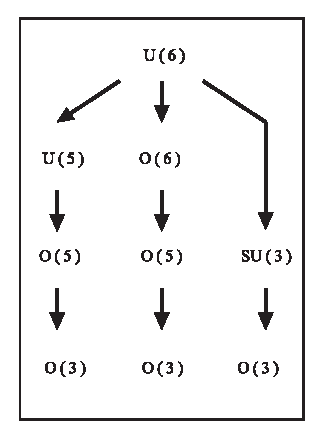
\includegraphics[scale=.65]{figure}
%
% If no graphics program available, insert a blank space i.e. use
%\picplace{5cm}{2cm} % Give the correct figure height and width in cm
%
\caption{If the width of the figure is less than 7.8 cm use the \texttt{sidecapion} command to flush the caption on the left side of the page. If the figure is positioned at the top of the page, align the sidecaption with the top of the figure -- to achieve this you simply need to use the optional argument \texttt{[t]} with the \texttt{sidecaption} command}
\label{fig:1}       % Give a unique label
\end{figure}


\paragraph{Paragraph Heading} %
Instead of simply listing headings of different levels we recommend to
let every heading be followed by at least a short passage of text.
Further on please use the \LaTeX\ automatism for all your
cross-references and citations as has already been described in
Sect.~\ref{sec:2}.

Please note that the first line of text that follows a heading is not indented, whereas the first lines of all subsequent paragraphs are.

For typesetting numbered lists we recommend to use the \verb|enumerate| environment -- it will automatically render Springer's preferred layout.

\begin{enumerate}
\item{Livelihood and survival mobility are oftentimes coutcomes of uneven socioeconomic development.}
\begin{enumerate}
\item{Livelihood and survival mobility are oftentimes coutcomes of uneven socioeconomic development.}
\item{Livelihood and survival mobility are oftentimes coutcomes of uneven socioeconomic development.}
\end{enumerate}
\item{Livelihood and survival mobility are oftentimes coutcomes of uneven socioeconomic development.}
\end{enumerate}


\subparagraph{Subparagraph Heading} In order to avoid simply listing headings of different levels we recommend to let every heading be followed by at least a short passage of text. Use the \LaTeX\ automatism for all your cross-references and citations as has already been described in Sect.~\ref{sec:2}, see also Fig.~\ref{fig:2}.

For unnumbered list we recommend to use the \verb|itemize| environment -- it will automatically render Springer's preferred layout.

\begin{itemize}
\item{Livelihood and survival mobility are oftentimes coutcomes of uneven socioeconomic development, cf. Table~\ref{tab:1}.}
\begin{itemize}
\item{Livelihood and survival mobility are oftentimes coutcomes of uneven socioeconomic development.}
\item{Livelihood and survival mobility are oftentimes coutcomes of uneven socioeconomic development.}
\end{itemize}
\item{Livelihood and survival mobility are oftentimes coutcomes of uneven socioeconomic development.}
\end{itemize}

\begin{figure}[t]
\sidecaption[t]
% Use the relevant command for your figure-insertion program
% to insert the figure file.
% For example, with the option graphics use
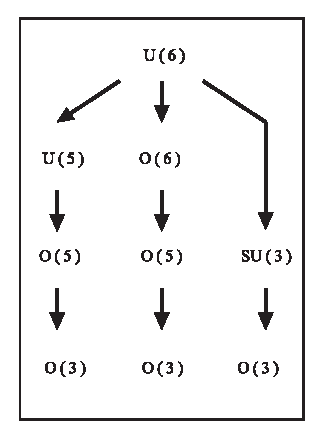
\includegraphics[scale=.65]{figure}
%
% If no graphics program available, insert a blank space i.e. use
%\picplace{5cm}{2cm} % Give the correct figure height and width in cm
%
%\caption{Please write your figure caption here}
\caption{If the width of the figure is less than 7.8 cm use the \texttt{sidecapion} command to flush the caption on the left side of the page. If the figure is positioned at the top of the page, align the sidecaption with the top of the figure -- to achieve this you simply need to use the optional argument \texttt{[t]} with the \texttt{sidecaption} command}
\label{fig:2}       % Give a unique label
\end{figure}

\runinhead{Run-in Heading Boldface Version} Use the \LaTeX\ automatism for all your cross-references and citations as has already been described in Sect.~\ref{sec:2}.

\subruninhead{Run-in Heading Italic Version} Use the \LaTeX\ automatism for all your cross-refer\-ences and citations as has already been described in Sect.~\ref{sec:2}\index{paragraph}.
% Use the \index{} command to code your index words
%
% For tables use
%
\begin{table}
\caption{Please write your table caption here}
\label{tab:1}       % Give a unique label
%
% Follow this input for your own table layout
%
\begin{tabular}{p{2cm}p{2.4cm}p{2cm}p{4.9cm}}
\hline\noalign{\smallskip}
Classes & Subclass & Length & Action Mechanism  \\
\noalign{\smallskip}\svhline\noalign{\smallskip}
Translation & mRNA$^a$  & 22 (19--25) & Translation repression, mRNA cleavage\\
Translation & mRNA cleavage & 21 & mRNA cleavage\\
Translation & mRNA  & 21--22 & mRNA cleavage\\
Translation & mRNA  & 24--26 & Histone and DNA Modification\\
\noalign{\smallskip}\hline\noalign{\smallskip}
\end{tabular}
$^a$ Table foot note (with superscript)
\end{table}
%
\section{Section Heading}
\label{sec:3}
% Always give a unique label
% and use \ref{<label>} for cross-references
% and \cite{<label>} for bibliographic references
% use \sectionmark{}
% to alter or adjust the section heading in the running head
Instead of simply listing headings of different levels we recommend to
let every heading be followed by at least a short passage of text.
Further on please use the \LaTeX\ automatism for all your
cross-references and citations as has already been described in
Sect.~\ref{sec:2}.

Please note that the first line of text that follows a heading is not indented, whereas the first lines of all subsequent paragraphs are.

If you want to list definitions or the like we recommend to use the Springer-enhanced \verb|description| environment -- it will automatically render Springer's preferred layout.

\begin{description}[Type 1]
\item[Type 1]{That addresses central themes pertainng to migration, health, and disease. In Sect.~\ref{sec:1}, Wilson discusses the role of human migration in infectious disease distributions and patterns.}
\item[Type 2]{That addresses central themes pertainng to migration, health, and disease. In Sect.~\ref{subsec:2}, Wilson discusses the role of human migration in infectious disease distributions and patterns.}
\end{description}

\subsection{Subsection Heading} %
In order to avoid simply listing headings of different levels we recommend to let every heading be followed by at least a short passage of text. Use the \LaTeX\ automatism for all your cross-references and citations citations as has already been described in Sect.~\ref{sec:2}.

Please note that the first line of text that follows a heading is not indented, whereas the first lines of all subsequent paragraphs are.

\begin{svgraybox}
If you want to emphasize complete paragraphs of texts we recommend to use the newly defined Springer class option \verb|graybox| and the newly defined environment \verb|svgraybox|. This will produce a 15 percent screened box 'behind' your text.

If you want to emphasize complete paragraphs of texts we recommend to use the newly defined Springer class option and environment \verb|svgraybox|. This will produce a 15 percent screened box 'behind' your text.
\end{svgraybox}


\subsubsection{Subsubsection Heading}
Instead of simply listing headings of different levels we recommend to
let every heading be followed by at least a short passage of text.
Further on please use the \LaTeX\ automatism for all your
cross-references and citations as has already been described in
Sect.~\ref{sec:2}.

Please note that the first line of text that follows a heading is not indented, whereas the first lines of all subsequent paragraphs are.

\begin{theorem}
Theorem text goes here.
\end{theorem}
%
% or
%
\begin{definition}
Definition text goes here.
\end{definition}

\begin{proof}
%\smartqed
Proof text goes here.
\qed
\end{proof}

\paragraph{Paragraph Heading} %
Instead of simply listing headings of different levels we recommend to
let every heading be followed by at least a short passage of text.
Further on please use the \LaTeX\ automatism for all your
cross-references and citations as has already been described in
Sect.~\ref{sec:2}.

Note that the first line of text that follows a heading is not indented, whereas the first lines of all subsequent paragraphs are.
%
% For built-in environments use
%
\begin{theorem}
Theorem text goes here.
\end{theorem}
%
\begin{definition}
Definition text goes here.
\end{definition}
%
\begin{proof}
\smartqed
Proof text goes here.
\qed
\end{proof}
%
\begin{acknowledgement}
If you want to include acknowledgments of assistance and the like at the end of an individual chapter please use the \verb|acknowledgement| environment -- it will automatically render Springer's preferred layout.
\end{acknowledgement}
%
\section*{Appendix}
\addcontentsline{toc}{section}{Appendix}
%
%
When placed at the end of a chapter or contribution (as opposed to at the end of the book), the numbering of tables, figures, and equations in the appendix section continues on from that in the main text. Hence please \textit{do not} use the \verb|appendix| command when writing an appendix at the end of your chapter or contribution. If there is only one the appendix is designated ``Appendix'', or ``Appendix 1'', or ``Appendix 2'', etc. if there is more than one.

\begin{equation}
a \times b = c
\end{equation}

%%%%%%%%%%%%%%%%%%%%%%%% referenc.tex %%%%%%%%%%%%%%%%%%%%%%%%%%%%%%
% sample references
% %
% Use this file as a template for your own input.
%
%%%%%%%%%%%%%%%%%%%%%%%% Springer-Verlag %%%%%%%%%%%%%%%%%%%%%%%%%%
%
% BibTeX users please use
% \bibliographystyle{}
% \bibliography{}
%
\biblstarthook{References may be \textit{cited} in the text either by number (preferred) or by author/year.\footnote{Make sure that all references from the list are cited in the text. Those not cited should be moved to a separate \textit{Further Reading} section or chapter.} The reference list should ideally be \textit{sorted} in alphabetical order -- even if reference numbers are used for the their citation in the text. If there are several works by the same author, the following order should be used: 
\begin{enumerate}
\item all works by the author alone, ordered chronologically by year of publication
\item all works by the author with a coauthor, ordered alphabetically by coauthor
\item all works by the author with several coauthors, ordered chronologically by year of publication.
\end{enumerate}
The recommended style for references\footnote{Always use the standard abbreviation of a journal's name according to the ISSN \textit{List of Title Word Abbreviations}.} is depicted in ~\cite{science-contrib, science-online, science-mono, science-journal, science-DOI}.
}

\begin{thebibliography}{99.}%
% and use \bibitem to create references.
%
% Use the following syntax and markup for your references if 
% the subject of your book is from the field 
% "Mathematics, Physics, Statistics, Computer Science"
%
% Contribution 
\bibitem{science-contrib} Broy, M.: Software engineering --- from auxiliary to key technologies. In: Broy, M., Dener, E. (eds.) Software Pioneers, pp. 10-13. Springer, Heidelberg (2002)
%
% Online Document
\bibitem{science-online} Dod, J.: Effective substances. In: The Dictionary of Substances and Their Effects. Royal Society of Chemistry (1999) Available via DIALOG. \\
\url{http://www.rsc.org/dose/title of subordinate document. Cited 15 Jan 1999}
%
% Monograph
\bibitem{science-mono} Geddes, K.O., Czapor, S.R., Labahn, G.: Algorithms for Computer Algebra. Kluwer, Boston (1992) 
%
% Journal article
\bibitem{science-journal} Hamburger, C.: Quasimonotonicity, regularity and duality for nonlinear systems of partial differential equations. Ann. Mat. Pura. Appl. \textbf{169}, 321--354 (1995)
%
% Journal article by DOI
\bibitem{science-DOI} Slifka, M.K., Whitton, J.L.: Clinical implications of dysregulated cytokine production. J. Mol. Med. (2000) doi: 10.1007/s001090000086 
%
\end{thebibliography}

\end{document}
